\chapter{Difração da luz}
\textsl{{\sffamily(Versão: \today)}}
Um dos argumentos invocados por Newton na sua oposição à teoria da natureza
ondulatória da luz foi o da propagação retilínea. Com efeito, dizia Newton, os
fenómenos ondulatórios não se propagam sempre em linha reta. Por exemplo,
podemos ouvir alguém que nos fala de detrás de uma árvore, e as ondulações da
superfície do mar ou dos lagos não ficam totalmente bloqueadas por ilhas (ver a
Figura~\ref{fig:40-070}).
\begin{figure}[htb]
    \begin{center}
        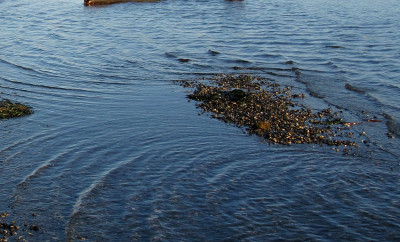
\includegraphics{figs/f40-070.jpg}
        \caption{Difração de ondas na superfície de um lago em torno de
            uma ilhota de cascalho (fonte:
            \protect\url{http://gravelbeach.blogspot.pt/2011/12/ala-spit_15.html}).
        \label{fig:40-070} }
\end{center}
\end{figure}
Estas ondas (pelo menos as de
som e as do mar), têm a capacidade de se encurvarem, rodeando parcial ou
totalmente os obstáculos que encontram no seu caminho, efeito que tem o nome de
\emph{difração}. Ora, dizia ainda Newton, nada de parecido se podia observar
para a luz, pelo que ela não podia, assim, ser considerada como um fenómeno
ondulatório. 

Mas a verdade é que a luz apresenta também fenómenos de difração, embora com
muito menor intensidade do que o som ou as ondas do mar, pelo menos em condições
habituais. Nesta secção estudaremos a difração da luz na passagem através de uma
fenda fina aberta num obstáculo opaco. O ponto de partida é o princípio de
Huyghens: cada ponto numa frente de onda é fonte de ondas esféricas que
interferem mutuamente no avanço da frente de onda. Ou seja, o valor da função de
onda em cada ponto e em cada instante é o que resulta da sobreposição das ondas
originadas nos vários pontos da frente de onda em instantes anteriores.

\section{Difração da luz numa fenda simples}
Consideremos então radiação que incide num obstáculo opaco, onde se abriu uma
fenda com largura $a$, centrada na origem (ver a Figura~\ref{fig:oof110}).
Pretende-se determinar a função de onda difratada numa direção que faz com
a direção de incidência (o eixo dos $x$, na figura) um ângulo $\theta$.
\begin{figure}[htb]
    \begin{center}
        \small
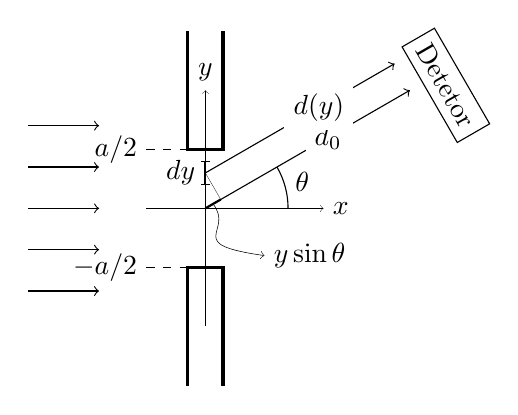
\begin{tikzpicture}[scale=1.5]
\draw [ultra thin, ->](-0.5,0)--(1,0) node [right]{$x$};
\draw [ultra thin, ->](0,-1.)--(0,1.) node [above]{$y$};
\draw [very thick](-0.15,-1.5) -- (-0.15,-0.5) -- (0.15,-0.5) -- (0.15,-1.5);
\draw [very thick](-0.15,1.5) -- (-0.15,0.5)--(0.15,0.5)--(0.15,1.5);
\draw [ultra thin, dashed] (-0.5,0.5) node [left] {$a/2$}--(-0.15,0.5);
\draw [ultra thin, dashed] (-0.5,-0.5) node [left] {$-a/2$}--(-0.15,-0.5);
\draw [->](0,0)--(30:2) node [pos=0.6,fill=white] {$d_0$};
\draw [->](0,0.3)--++(30:1.85) node[pos=0.6,fill=white] {$d(y)$};
\draw(-0.035,0.2)--(0.035,0.2);
\draw(-0.035,0.4)--(0.035,0.4);
\draw[thick](0,0.2)--(0,0.4) node[midway,left]{$dy$};
\node (D) at (1.8,1.45) [rotate=-60,right,draw] {Detetor};
\draw [ultra thin](0,0.3)--++(-60:0.26);
\draw [thick] (0,0)--(30:0.15);
\draw (0.7,0) arc (0:30:0.7);
\node at (15:0.85){$\theta$};
\draw [very thin, ->] ++(30:0.075) .. controls (0.25,-0.2) and (-0.2,-0.3) ..(0.5,-0.4) node [right]{$y\sin\theta$};
\draw [->] (-1.5, 0.70)--(-0.9,00.70);
\draw [->] (-1.5, 0.35)--(-0.9, 0.35);
\draw [->] (-1.5, 0.00)--(-0.9, 0.00);
\draw [->] (-1.5,-0.35)--(-0.9,-0.35);
\draw [->] (-1.5,-0.70)--(-0.9,-0.70);
\end{tikzpicture}
\end{center}
\caption{Difração por uma fenda simples.\label{fig:oof110}}
\end{figure}
Seja $d_0$ a distância que separa o centro da fenda do ponto onde queremos
determinar a função de onda e $d(y)$ a distância de um ponto da fenda com
ordenada $y$ até esse mesmo ponto. A contribuição que a porção infinitesimal de
fenda com comprimento $dy$ representada na figura dá para a função de onda no
ponto onde a queremos determinar é 
\begin{equation*}
    d\psi = \frac{A}{a}dy\cos\left(2\pi\left[\frac{d(y)}{\lambda}-\frac{t}{T}
    \right]\right),
\end{equation*}
onde $A$ é um fator proporcional à amplitude da onda incidente\footnote{Este
    fator depende ainda de outras variáveis, nomeadamente a distância ao
    detetor, mas que não queremos agora considerar. O que queremos, de facto,
    enfatizar, é que a amplitude da onda difratada na fenda é, em qualquer ponto
do espaço, proporcional à amplitude da onda incidente.}, e $\lambda$ e $T$ são, respetivamente,
o comprimento de onda e o período dessa onda e escolhemos nula a constante de
fase.  Mas $d(y)=d_0-y\sin\theta$. Então
\begin{equation}
    d\psi = \frac{A}{a} dy\cos\left[\Omega(t)-\strut\phi(y)\right],\label{eq:oo010}
\end{equation}
tendo-se introduzido os símbolos
\begin{align*}
    \Omega(t)&=2\pi\left(\frac{d_0}{\lambda}-\frac{t}{T}\right)&
    \phi(y)&=2\pi \frac y \lambda \sin\theta
\end{align*}
para aligeirar a notação. A função de onda resultante no ponto onde a queremos
calcular é a soma de um número infinito de contribuições semelhantes à da
eq.~\eqref{eq:oo010}, uma por cada ponto da frente de onda que atravessa a
abertura, ou seja, uma por cada ponto do eixo dos $y$ no intervalo
$[-a/2,\,a/2]$, ou seja ainda,
\begin{equation*}
    \psi=\int_{-a/2}^{a/2}\frac{A}{a}\cos\left[\strut\Omega(t)-\phi(y)\right]dy.
\end{equation*}
Usando a igualdade trigonométrica $\cos(a+b)=\cos a\cos b-\sin a\sin b$, este
integral pode escrever-se como
\begin{equation*}
    \psi=\frac{A}{a}\cos\Omega(t)\int_{-a/2}^{a/2}\cos\phi(y)\,dy+
         \frac{A}{a}\cos\Omega(t)\int_{-a/2}^{a/2}\sin\phi(y)\,dy,
\end{equation*}
uma vez que como o termo $\Omega(t)$ não depende de $y$, $\cos\Omega$ e
$\sin\Omega$ podem ser postos em evidência nos respetivos integrais. Seja agora
$\mu=2\pi/\lambda\;\sin\theta$. Então, para o primeiro destes integrais temos
\begin{align*}
    \int_{-a/2}^{a/2}\cos\phi\,dy&=\int_{-a/2}^{a/2}\cos\mu y\,dy=
    \left[\frac{1}{\mu}\sin\mu y\right]_{-a/2}^{a/2}=
    \frac2{\mu}\sin\frac{\mu a}2.
\end{align*}
Da mesma maneira, para o segundo,
\begin{align*}
    \int_{-a/2}^{a/2}\sin\phi\,dy&=\int_{-a/2}^{a/2}\sin\mu y\,dy=
    \left[\frac{1}{\mu}\cos\mu y\right]_{-a/2}^{a/2}=0.
\end{align*}
Juntando estes dois resultados, obtemos, por fim,
\begin{equation*}
    \psi = A\,\frac{\sin(\mu a/2)}{\mu a/2}\,\cos\Omega(t).
\end{equation*}
Esta equação mostra que a natureza da onda não se altera quando atravessa a
fenda, no sentido em que o seu comprimento de onda e período se mantêm (recorde
que estes parâmetros estão integrados no termo $\Omega(t)$). No entanto, a
direção de propagação deixa de ser única. Em vez disso, nota-se agora que a onda
se espalha num leque de direções, tendo uma amplitude variável dada por
\begin{equation*}
    A(\theta)=A\frac{\sin(\mu a/2)}{\mu
    a/2}=Aj_0(\pi\frac{a}{\lambda}\sin\theta),
\end{equation*}
onde se introduziu a chamada \emph{função esférica de Bessel de ordem zero}
$j_0(x)=\sin x/x$. A intensidade do sinal ondulatório, que, como vimos, é
proporcional ao quadrado da amplitude, é então
\begin{equation}
    I(\theta)= I_0 j_0^2(\pi\frac{a}{\lambda}\sin\theta),
\end{equation}
onde $I_0=I(\theta=0)$. A Figura~\ref{fig:oof120} mostra o gráfico da
intensidade da difração como função do ângulo da direção da radiação difratada,
para dois valores diferentes do quociente entre a largura da fenda e o
comprimento de onda.
\begin{figure}[htb]
\begin{center}
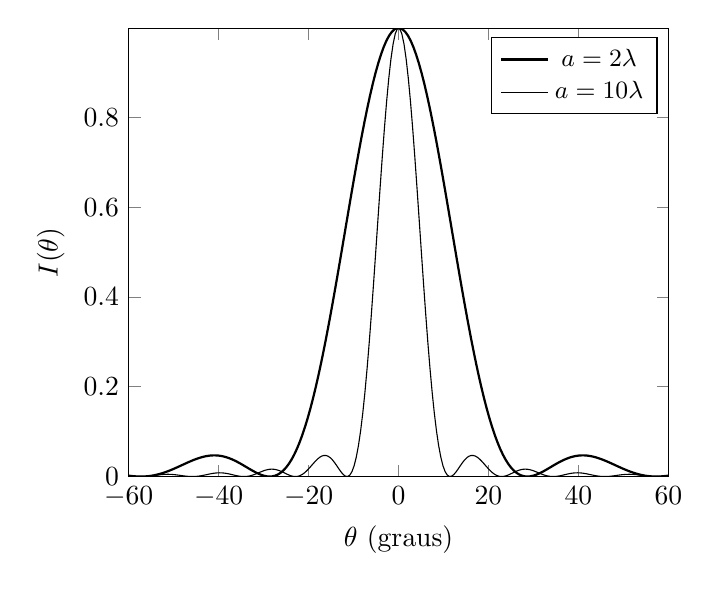
\begin{tikzpicture}
    \begin{axis}[
        enlargelimits=false,
        xlabel=$\theta$ (graus),
        ylabel=$I(\theta)$]
        \addplot [
            domain=-60:60,
            samples=200,thick
            ] {(sin(2*pi*x)/(2*pi^2*x/180))^2};
        \addlegendentry{\small $a=2\lambda$}
        \addplot [
            domain=-60:60,
            samples=250
            ] {(sin(5*pi*x)/(5*x*pi^2/180))^2};
        \addlegendentry{\small $a=10\lambda$}
    \end{axis}
\end{tikzpicture}
\caption{Intensidade da radiação difratada numa fenda simples como função do
ângulo da direção de difração (medido a partir da direção de incidência), para
$a=2\lambda$ e $a=10\lambda$.%
\label{fig:oof120}}
\end{center}
\end{figure}
Pode ver-se que a intensidade é máxima para $\theta=0$, ou seja na direção de
incidência, como seria de esperar intuitivamente, e que se reduz para zero,
tanto mais rapidamente quanto maior for a largura da abertura. A intensidade
atinge um primeiro valor mínimo mas depois apresenta oscilações com amplitude
sucessivamente menor à medida que o ângulo aumenta. Os vários mínimos de
intensidade ocorrem para ângulos $\theta_k$ dados por
\begin{equation*}
    \frac{\displaystyle%
    \sin\left(\pi\frac a \lambda \sin\theta_k\right)}{%
    \displaystyle \pi\frac a \lambda \sin\theta_k}=0.
\end{equation*}
Esta igualdade é satisfeita quando o numerador da fração se anula, sem se anular
o denominador\footnote{Se os dois --- numerador e denominador --- se anulam,
temos uma indeterminação do tipo 0/0, que, uma vez levantada, se revela
representar o valor máximo da função, em $\theta=0$!}, ou seja para
\begin{equation*}
    \pi \frac a \lambda\sin\theta_k=k\pi,\quad k=\pm1,\;\pm2,\;\pm3,\;\ldots.
\end{equation*}
O primeiro mínimo, em particular, ocorre numa direcção que faz com a de
incidência um ângulo de 
\begin{equation*}
    \theta_1 = \arcsin\frac{\lambda}{a}.
\end{equation*}
Assim, constatamos que se a largura da fenda é muito maior do que o comprimento
de onda (como certamente é o caso quando tratamos com luz e fendas ``normais,''
como janelas em paredes), então o ângulo do primeiro mínimo, que podemos tomar
como medida do espalhamento por difração, é muito pequeno, é praticamente zero.
Por isso é que não se notam, no dia a dia, efeitos da difração da luz. Mas ela
existe e pode ser demonstrada em experiências relativamente simples. Por
exemplo, a Figura~\ref{fig:40-080} mostra a sombra de uma lâmina de barbear
iluminada com raios laser. São aí claramente visíveis vários mínimos de
difração, na forma de contornos escuros em torno da sombra da lâmina.
\begin{figure}[htb]
    \begin{center}
        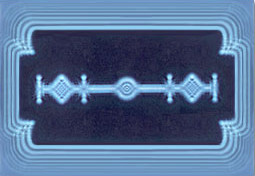
\includegraphics[width=0.3\textwidth]{figs/f40-080.jpg}
    \end{center}
    \caption{Difração de luz laser numa lâmina de barbear. (Fonte:
        \protect%
        \url{http://micro.magnet.fsu.edu/primer/lightandcolor/diffractionintro.html})%
    \label{fig:40-080}}
\end{figure}

\section{Difração num obstáculo retangular}
\tobedone{}

\section{Redes de difração 2}
\tobedone{}

\section{Difração numa janela circular}
\tobedone{}

\section{Lentes difrativas}
\tobedone{}
